%%%%%%%%%%%%%%%%%%%%%%%%%%%%%%%%%%%%%%%%%%%%%%%%%%%%%%%%%%%%%%%%%%%%%%%%%%%%%%%%%%%%%%%
% ĐỀ KIỂM TRA GIỮA HỌC KÌ I - TOÁN 12 - NĂM HỌC 2025-2026
% Trường THPT Lý Tự Trọng - Sở GD&ĐT Đà Nẵng (đề gồm 6 trang, đáp án 13 trang)
%
% Chuyển từ Word (MathType) sang LaTeX theo cấu trúc file:
%   D:\Tailieu\dataDT\12-OTC\2-D1B5-SO-15-2425_2.tex
%
% GHI CHÚ QUAN TRỌNG
% 1) Toàn bộ công thức trong file Word gốc là ảnh WMF/OLE (MathType) nên không trích xuất
%    được dạng text - đã được đọc từ bản render và gõ lại bằng LaTeX.
% 2) Các HÌNH VẼ (bảng biến thiên, đồ thị, hình học) được tách nguyên bản từ file Word và
%    chèn bằng \includegraphics, lưu tại: hinhve/GK1-12-LTT/
%      cau01-bbt.png, cau02-bbt.png, cau03-bbt.png, cau12-bbt.png, cau15-bbt.png,
%      cau18-bbt.png, cau19-bbt.png ................ (bảng biến thiên)
%      cau04-do-thi.png, cau05-do-thi.png, cau07-do-thi.png, cau08-do-thi.png,
%      cau09-do-thi.png, cau10-do-thi.png, cau13-do-thi.png, cau19-do-thi.png (đồ thị)
%      cau16-hinh-hoc.png, cau16-loi-giai-hinh-thang.png, cau17-hinh-hoc.png (hình học)
%    (Có thể chuyển các bảng biến thiên sang tkz-tab nếu muốn đồng bộ với các file khác.)
% 3) Cấu trúc: \TN (12 câu) - \TNTF (2 câu Đ/S) - \TNSA (4 câu trả lời ngắn) - \TL (3 bài tự luận).
%    Lời giải dùng \loigiai{} nên in được cả đề (chạy \anLG) và lời giải (\hienLG).
% 4) Bảng đáp án: \inputansbox{12,2,4}{ans/ans\currfilebase}
%
% Phân bố đáp án (đối chiếu nhanh):
%   PHẦN I:  1.C  2.B  3.B  4.B  5.B  6.A  7.C  8.C  9.D  10.D  11.D  12.B
%   PHẦN II: Câu 13: a) S - b) Đ - c) S - d) Đ        Câu 14: a) Đ - b) S - c) Đ - d) S
%   PHẦN III: 15) 14    16) 1,07    17) 0,30    18) 521
%   PHẦN IV: 19) khảo sát y=-x^3+3x^2-4    20) max=10, min=-186    21) v(4)=105
%
% LƯU Ý: chỉ câu 3 trong file gốc không có phần hướng dẫn giải chi tiết (chỉ ghi "Chọn B"),
% đã được ghi rõ bằng comment %(nguồn không có lời giải chi tiết) và bổ sung 1 dòng lập luận ngắn.
% Đã build thử bằng preamble cautrucDT + ex_test v3.3.4: 10 trang, bảng đáp án khớp.
%%%%%%%%%%%%%%%%%%%%%%%%%%%%%%%%%%%%%%%%%%%%%%%%%%%%%%%%%%%%%%%%%%%%%%%%%%%%%%%%%%%%%%%

\begin{name}
	{\tenchude}
	{ĐỀ KIỂM TRA GIỮA HỌC KÌ I - TOÁN 12}
	{THPT LÝ TỰ TRỌNG - ĐÀ NẴNG}
	{Thời gian làm bài 90 phút, không kể thời gian giao đề}
\end{name}

\TN
\Opensolutionfile{ans}[ans/ans\currfilebase]

%%%=============Câu 1=============%%%
\begin{ex}%[GK1, THPT Lý Tự Trọng - Đà Nẵng, 2025-2026]%[VNPmath]%[2D1N2-1]
	Cho hàm số $y=f(x)$ có bảng biến thiên như sau
	\begin{center}
		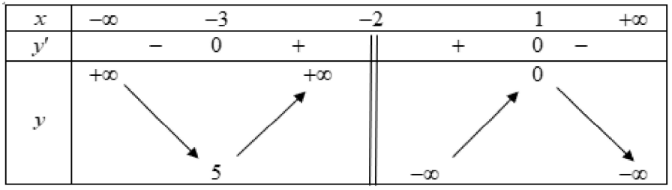
\includegraphics[width=0.62\linewidth]{hinhve/GK1-12-LTT/cau01-bbt.png}
	\end{center}
	Giá trị cực đại của hàm số $y=f(x)$ bằng
	\choice
	{$1$}
	{$5$}
	{\True $0$}
	{$-3$}
	\loigiai{
		Từ bảng biến thiên ta thấy hàm số $y=f(x)$ đạt cực đại tại $x=1$, $y_{\text{CĐ}}=0$.
	}
\end{ex}

%%%=============Câu 2=============%%%
\begin{ex}%[GK1, THPT Lý Tự Trọng - Đà Nẵng, 2025-2026]%[VNPmath]%[2D1N3-1]
	Cho hàm số $y=f(x)$ liên tục và có bảng biến thiên trên đoạn $[-1;3]$ như hình bên dưới. Giá trị lớn nhất của hàm số trên đoạn $[-1;3]$ bằng
	\begin{center}
		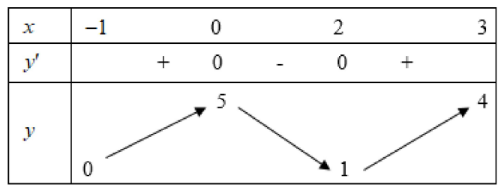
\includegraphics[width=0.6\linewidth]{hinhve/GK1-12-LTT/cau02-bbt.png}
	\end{center}
	\choice
	{$4$}
	{\True $5$}
	{$1$}
	{$0$}
	\loigiai{
		Từ bảng biến thiên ta có $\max\limits_{[-1;3]} f(x)=f(0)=5$.
	}
\end{ex}

%%%=============Câu 3=============%%%
\begin{ex}%[GK1, THPT Lý Tự Trọng - Đà Nẵng, 2025-2026]%[VNPmath]%[2D1N1-1]
	Cho hàm số $y=f(x)$ xác định trên $\mathbb{R}$ và có bảng biến thiên như sau
	\begin{center}
		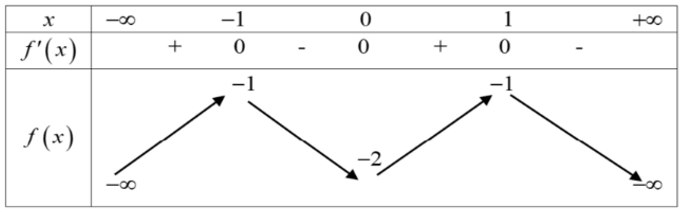
\includegraphics[width=0.62\linewidth]{hinhve/GK1-12-LTT/cau03-bbt.png}
	\end{center}
	Hàm số $y=f(x)$ nghịch biến trên khoảng nào dưới đây?
	\choice
	{$(-\infty;0)$}
	{\True $(-1;0)$}
	{$(-1;1)$}
	{$(0;1)$}
	\loigiai{
		%(nguồn không có lời giải chi tiết)
		Từ bảng biến thiên ta thấy $f'(x)<0$ trên các khoảng $(-1;0)$ và $(1;+\infty)$ nên hàm số nghịch biến trên các khoảng đó.
	}
\end{ex}

%%%=============Câu 4=============%%%
\begin{ex}%[GK1, THPT Lý Tự Trọng - Đà Nẵng, 2025-2026]%[VNPmath]%[2D1N2-2]
	Cho hàm số $y=f(x)$ có đồ thị như hình vẽ sau
	\begin{center}
		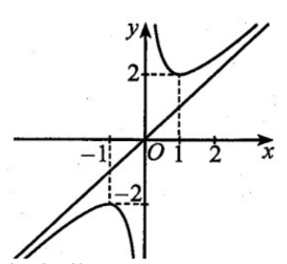
\includegraphics[width=0.38\linewidth]{hinhve/GK1-12-LTT/cau04-do-thi.png}
	\end{center}
	Điểm cực đại của đồ thị hàm số đã cho là
	\choice
	{$(-2;-1)$}
	{\True $(1;2)$}
	{$(-1;-2)$}
	{$(2;1)$}
	\loigiai{
		Từ hình vẽ, đồ thị hàm số có điểm cực đại là $(1;2)$.
	}
\end{ex}

%%%=============Câu 5=============%%%
\begin{ex}%[GK1, THPT Lý Tự Trọng - Đà Nẵng, 2025-2026]%[VNPmath]%[2D1H3-1]
	Cho hàm số $f(x)$ liên tục trên $[-1;5]$ và có đồ thị trên đoạn $[-1;5]$ như hình vẽ bên dưới. Giá trị nhỏ nhất của hàm số $f(x)$ trên đoạn $[-1;5]$ bằng
	\begin{center}
		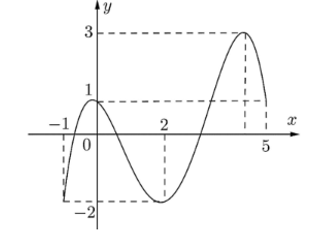
\includegraphics[width=0.42\linewidth]{hinhve/GK1-12-LTT/cau05-do-thi.png}
	\end{center}
	\choice
	{$2$}
	{\True $-2$}
	{$1$}
	{$3$}
	\loigiai{
		Từ đồ thị hàm số ta thấy $\min\limits_{[-1;5]} f(x)=-2$ khi $x=-1$ hoặc $x=2$.
	}
\end{ex}

%%%=============Câu 6=============%%%
\begin{ex}%[GK1, THPT Lý Tự Trọng - Đà Nẵng, 2025-2026]%[VNPmath]%[2D1N4-1]
	Đường tiệm cận đứng và tiệm cận ngang của đồ thị hàm số $y=\dfrac{2x-5}{4-x}$ có phương trình là
	\choice
	{\True $x=4;y=-2$}
	{$x=4;y=\dfrac{1}{2}$}
	{$x=4;y=5$}
	{$x=-4;y=-2$}
	\loigiai{
		Tập xác định của hàm số là $D=\mathbb{R}\setminus\{4\}$.\\
		Ta có $\lim\limits_{x\to\pm\infty} y=\lim\limits_{x\to\pm\infty}\dfrac{2x-5}{4-x}=\lim\limits_{x\to\pm\infty}\dfrac{2-\dfrac{5}{x}}{\dfrac{4}{x}-1}=-2$.\\
		$\lim\limits_{x\to 4^+} y=\lim\limits_{x\to 4^+}\dfrac{2x-5}{4-x}=-\infty$.\\
		Vậy đồ thị hàm số có tiệm cận ngang $y=-2$, tiệm cận đứng $x=4$.
	}
\end{ex}

%%%=============Câu 7=============%%%
\begin{ex}%[GK1, THPT Lý Tự Trọng - Đà Nẵng, 2025-2026]%[VNPmath]%[2D1N4-1]
	Cho hàm số $y=f(x)$ liên tục và có đồ thị như hình vẽ.
	\begin{center}
		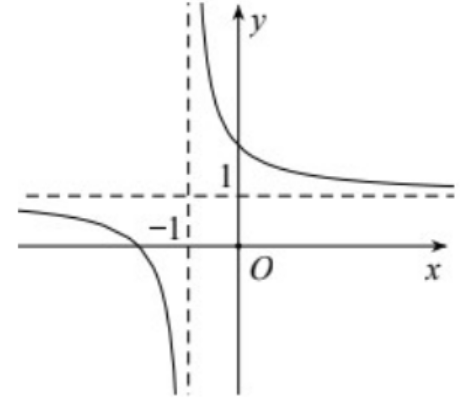
\includegraphics[width=0.42\linewidth]{hinhve/GK1-12-LTT/cau07-do-thi.png}
	\end{center}
	Đường tiệm cận ngang của đồ thị có phương trình nào sau đây?
	\choice
	{$x=1$}
	{$x=-1$}
	{\True $y=1$}
	{$y=-1$}
	\loigiai{
		Dựa vào đồ thị hàm số ta có đường tiệm cận ngang của đồ thị có phương trình là $y=1$.
	}
\end{ex}

%%%=============Câu 8=============%%%
\begin{ex}%[GK1, THPT Lý Tự Trọng - Đà Nẵng, 2025-2026]%[VNPmath]%[2D1H5-3]
	Hàm số nào dưới đây có đồ thị như hình vẽ sau?
	\begin{center}
		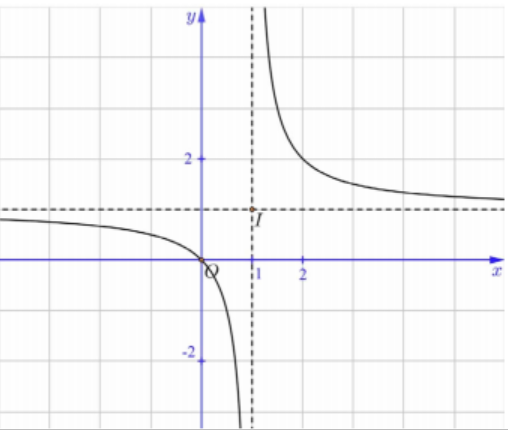
\includegraphics[width=0.42\linewidth]{hinhve/GK1-12-LTT/cau08-do-thi.png}
	\end{center}
	\choice
	{$y=x^3-3x+2$}
	{$y=\dfrac{x^2-4x+5}{x-2}$}
	{\True $y=\dfrac{x}{x-1}$}
	{$y=-x^3+3x^2-1$}
	\loigiai{
		Dựa vào đồ thị hàm số ta có đường tiệm cận ngang là $y=1$, tiệm cận đứng là $x=1$ suy ra hàm số có đồ thị như hình trên là $y=\dfrac{x}{x-1}$.
	}
\end{ex}

%%%=============Câu 9=============%%%
\begin{ex}%[GK1, THPT Lý Tự Trọng - Đà Nẵng, 2025-2026]%[VNPmath]%[2D1H5-3]
	Đường cong như hình vẽ dưới đây là đồ thị của hàm số nào?
	\begin{center}
		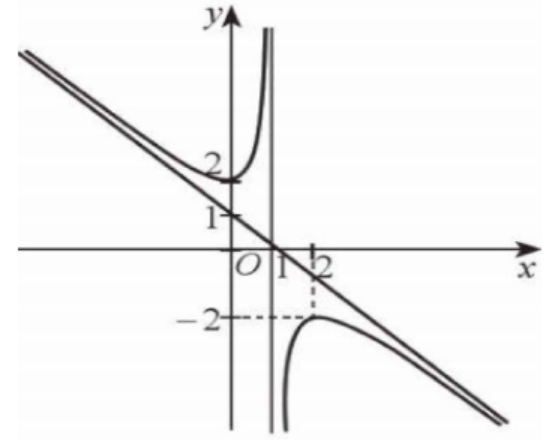
\includegraphics[width=0.46\linewidth]{hinhve/GK1-12-LTT/cau09-do-thi.png}
	\end{center}
	\choice
	{$y=\dfrac{1}{3}x^3-x^2-4$}
	{$y=-\dfrac{1}{3}x^3+3x^2-1$}
	{$y=\dfrac{2x-2}{3x-1}$}
	{\True $y=\dfrac{-x^2+2x-2}{x-1}$}
	\loigiai{
		Dựa vào đồ thị hàm số ta có tiệm cận đứng là $x=1$ nên ta loại trừ phương án $A$, $B$.\\
		Đồ thị đi qua điểm $A(2;-2)$ chỉ có đáp án $D$ thoả mãn.
	}
\end{ex}

%%%=============Câu 10=============%%%
\begin{ex}%[GK1, THPT Lý Tự Trọng - Đà Nẵng, 2025-2026]%[VNPmath]%[2D1H1-1]
	Cho hàm số $y=f(x)=ax^3+bx^2+cx+d\,(a\neq 0)$ có đồ thị như hình vẽ dưới đây.
	\begin{center}
		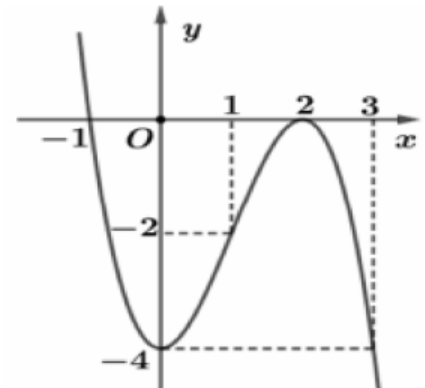
\includegraphics[width=0.42\linewidth]{hinhve/GK1-12-LTT/cau10-do-thi.png}
	\end{center}
	Hàm số $y=f(x)$ đồng biến trên khoảng nào dưới đây?
	\choice
	{$(-\infty;0)$}
	{$(-1;2)$}
	{$(2;+\infty)$}
	{\True $(0;2)$}
	\loigiai{
		Dựa vào đồ thị hàm số ta có hàm số $y=f(x)$ đồng biến trên khoảng $(0;2)$.
	}
\end{ex}

%%%=============Câu 11=============%%%
\begin{ex}%[GK1, THPT Lý Tự Trọng - Đà Nẵng, 2025-2026]%[VNPmath]%[2D1H4-2]
	Cho hàm số $y=\dfrac{2x^2-3x-1}{x-2}$. Tiệm cận xiên của đồ thị hàm số là đường thẳng
	\choice
	{$y=2x+3$}
	{$y=2x-1$}
	{$y=2x-3$}
	{\True $y=2x+1$}
	\loigiai{
		Ta có $y=\dfrac{2x^2-3x-1}{x-2}=2x+1+\dfrac{1}{x-2}$.\\
		Ta có $\lim\limits_{x\to+\infty}\left(f(x)-(2x+1)\right)=0$; $\lim\limits_{x\to-\infty}\left(f(x)-(2x+1)\right)=0$ suy ra tiệm cận xiên của đồ thị hàm số là đường thẳng $y=2x+1$.
	}
\end{ex}

%%%=============Câu 12=============%%%
\begin{ex}%[GK1, THPT Lý Tự Trọng - Đà Nẵng, 2025-2026]%[VNPmath]%[2D1N4-1]
	Cho hàm số $y=f(x)$ liên tục và có bảng biến thiên như hình vẽ
	\begin{center}
		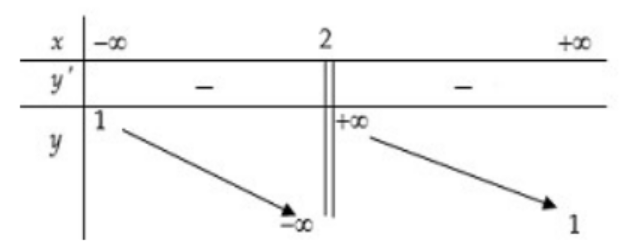
\includegraphics[width=0.62\linewidth]{hinhve/GK1-12-LTT/cau12-bbt.png}
	\end{center}
	Đường tiệm cận đứng của đồ thị có phương trình nào sau đây?
	\choice
	{$x=1$}
	{\True $x=2$}
	{$y=2$}
	{$y=1$}
	\loigiai{
		Dựa vào bảng biến thiên đề cho ta có $\lim\limits_{x\to 2^-} f(x)=-\infty$; $\lim\limits_{x\to 2^+} f(x)=+\infty$ suy ra đường tiệm cận đứng của đồ thị có phương trình $x=2$.
	}
\end{ex}

\TNTF

%%%=============Câu 13=============%%%
\begin{ex}%[GK1, THPT Lý Tự Trọng - Đà Nẵng, 2025-2026]%[VNPmath]%[2D1H4-3]
	Cho hàm số $y=\dfrac{ax+b}{cx-1}$ có đồ thị như hình vẽ sau:
	\begin{center}
		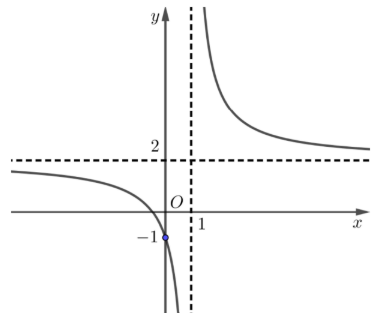
\includegraphics[width=0.42\linewidth]{hinhve/GK1-12-LTT/cau13-do-thi.png}
	\end{center}
	\choiceTF
	{Hàm số đã cho đồng biến trên khoảng $(-\infty;1)$ và $(1;+\infty)$}
	{\True Hàm số $y=f(x)=\dfrac{2x+1}{x-1}$}
	{$c=-1$}
	{\True Hàm số $y=f(x)$ không có cực trị}
	\loigiai{
		\begin{itemchoice}
		\itemch \textbf{Sai.}\\
		Từ hình vẽ ta thấy trên từng khoảng $(-\infty;1)$ và $(1;+\infty)$ thì đồ thị hàm số là một đường đi xuống tính từ trái sang phải nên hàm số nghịch biến trên các khoảng $(-\infty;1)$ và $(1;+\infty)$.
		\itemch \textbf{Đúng.}\\
		Từ hình vẽ ta thấy:
		\begin{itemize}
		\item Đồ thị hàm số có tiệm cận đứng là $x=1$ và tiệm cận ngang $y=2$.
		$$\Rightarrow\heva{&c\cdot 1-1=0\\&a\cdot 1+b\neq 0}\Leftrightarrow\heva{&c=1\\&a\neq -b.}$$
		\item Đồ thị hàm số có tiệm cận ngang $y=2$ $\Rightarrow\lim\limits_{x\to\pm\infty}\dfrac{ax+b}{cx-1}=\dfrac{a}{c}=2\Rightarrow a=2c=2$.
		\item Đồ thị hàm số cắt trục tung tại điểm có toạ độ $(0;-1)$ $\Rightarrow\dfrac{b}{-1}=-1\Leftrightarrow b=1$ (thoả mãn $a\neq -b$).
		\end{itemize}
		$\Rightarrow$ Hàm số $y=f(x)=\dfrac{2x+1}{x-1}$.
		\itemch \textbf{Sai.}\\
		Ta có $c=1$ (theo ý b).
		\itemch \textbf{Đúng.}\\
		Ta có $y'=\dfrac{-3}{(x-1)^2}<0,\forall x\neq 1$ $\Rightarrow$ Hàm số $y=f(x)$ không có cực trị.
		\end{itemchoice}
	}
\end{ex}

%%%=============Câu 14=============%%%
\begin{ex}%[GK1, THPT Lý Tự Trọng - Đà Nẵng, 2025-2026]%[VNPmath]%[2D1H4-2]
	Cho hàm số $(C)\colon y=f(x)=\dfrac{2x^2+3x-5}{x+3}$.
	\choiceTF
	{\True Đồ thị $(C)$ của hàm số không có đường tiệm cận ngang}
	{Giao điểm của 2 đường tiệm cận là $I(3;3)$}
	{\True Phương trình đường tiệm cận xiên của $(C)$ là $y=2x-3$}
	{Đường tiệm cận đứng của $(C)$ có phương trình $x=3$}
	\loigiai{
		\begin{itemchoice}
		\itemch \textbf{Đúng.}\\
		Ta có $\lim\limits_{x\to+\infty} f(x)=\lim\limits_{x\to+\infty}\dfrac{2x^2+3x-5}{x+3}=+\infty$ và $\lim\limits_{x\to-\infty} f(x)=\lim\limits_{x\to-\infty}\dfrac{2x^2+3x-5}{x+3}=-\infty$.\\
		$\Rightarrow$ đồ thị $(C)$ không có tiệm cận ngang.
		\itemch \textbf{Sai.}\\
		Ta có: $\lim\limits_{x\to(-3)^-} f(x)=\lim\limits_{x\to(-3)^-}\dfrac{2x^2+3x-5}{x+3}=+\infty$ và $\lim\limits_{x\to(-3)^+} f(x)=\lim\limits_{x\to(-3)^+}\dfrac{2x^2+3x-5}{x+3}=-\infty$.\\
		$\Rightarrow$ tiệm cận đứng $x=-3$.\\
		Ta có $(C)\colon y=\dfrac{2x^2+3x-5}{x+3}=2x-3+\dfrac{4}{x+3}$.\\
		Vì $\lim\limits_{x\to\pm\infty}\left[y-(2x-3)\right]=\lim\limits_{x\to\pm\infty}\dfrac{4}{x+3}=0$ $\Rightarrow$ tiệm cận xiên $y=2x-3$.\\
		Toạ độ giao điểm của 2 tiệm cận là nghiệm của hệ $\heva{&x=-3\\&y=2x-3}\Leftrightarrow\heva{&x=-3\\&y=-9.}$\\
		$\Rightarrow$ toạ độ giao điểm của hai tiệm cận là $I(-3;-9)$.
		\itemch \textbf{Đúng.}\\
		Đường tiệm cận xiên của $(C)$ có phương trình $y=2x-3$.
		\itemch \textbf{Sai.}\\
		Đường tiệm cận đứng của $(C)$ có phương trình $x=-3$.
		\end{itemchoice}
	}
\end{ex}

\TNSA

%%%=============Câu 15=============%%%
\begin{ex}%[GK1, THPT Lý Tự Trọng - Đà Nẵng, 2025-2026]%[VNPmath]%[2D1H2-1]
	Hàm số $y=\dfrac{x^2-x+1}{x-1}$ có giá trị cực đại và giá trị cực tiểu lần lượt là $a$ và $b$. Tính $a+5b$.
	\shortans{14}
	\loigiai{
		Đáp số: 14.\\
		TXĐ: $D=\mathbb{R}\setminus\{1\}$.\\
		$y=\dfrac{x^2-x+1}{x-1}=x+\dfrac{1}{x-1}\Rightarrow y'=1-\dfrac{1}{(x-1)^2}=0\Leftrightarrow\hoac{&x=2\\&x=0.}$\\
		BBT
		\begin{center}
			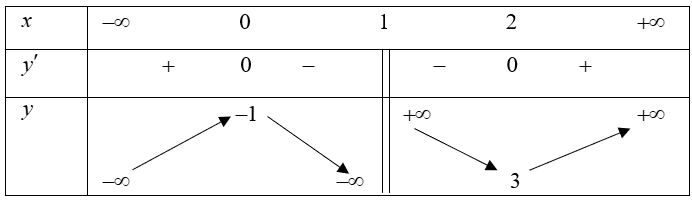
\includegraphics[width=0.62\linewidth]{hinhve/GK1-12-LTT/cau15-bbt.png}
		\end{center}
		Suy ra $a=-1$; $b=3$. Vậy $a+5b=14$.
	}
\end{ex}

%%%=============Câu 16=============%%%
\begin{ex}%[GK1, THPT Lý Tự Trọng - Đà Nẵng, 2025-2026]%[VNPmath]%[2H1V3-1]
	Một hình chóp cụt lục giác đều có thể tích là $\dfrac{7\sqrt{6}}{2}$, cạnh đáy lớn có độ dài gấp hai lần cạnh đáy nhỏ. Khi trải phẳng hình chóp cụt lục giác đều trên một mặt phẳng thì đáy lớn nội tiếp trên $1$ đường tròn (như hình vẽ). Tính độ dài cạnh đáy nhỏ của hình chóp cụt lục giác đều biết đường tròn ngoại tiếp đáy lớn có bán kính đạt giá trị nhỏ nhất (kết quả làm tròn đến hàng phần trăm).
	\begin{center}
		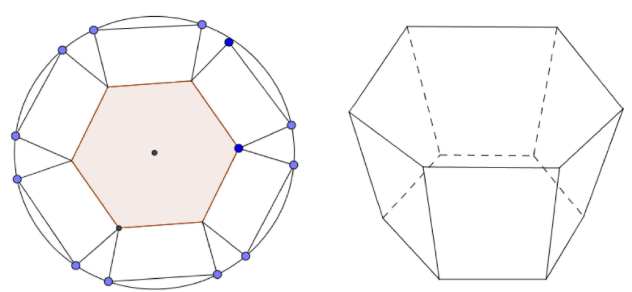
\includegraphics[width=0.72\linewidth]{hinhve/GK1-12-LTT/cau16-hinh-hoc.png}
	\end{center}
	\shortans{1{,}07}
	\loigiai{
		Đáp số: 1,07.\\
		Gọi độ dài cạnh đáy nhỏ là $x$.\\
		Độ dài cạnh đáy lớn là $2x$.\\
		Vì đáy là hình lục giác đều nên diện tích mặt đáy nhỏ là: $6\cdot\dfrac{x^2\sqrt{3}}{4}=\dfrac{3x^2\sqrt{3}}{2}$ (đvdt).\\
		Vì đáy là hình lục giác đều nên diện tích mặt đáy lớn là: $6\cdot\dfrac{(2x)^2\sqrt{3}}{4}=6x^2\sqrt{3}$ (đvdt).\\
		Khối hình chóp cụt lục giác đều có thể tích là $\dfrac{7\sqrt{6}}{2}$ nên chiều cao của hình chóp cụt là:
		$$h=\dfrac{7\sqrt{6}}{2}\cdot 3:\left(\dfrac{3x^2\sqrt{3}}{2}+6x^2\sqrt{3}+\sqrt{\dfrac{3x^2\sqrt{3}}{2}\cdot 6x^2\sqrt{3}}\right)=\dfrac{\sqrt{2}}{x^2}.$$
		Xét hình thang $ABDC$ với $AB=4x$, $CD=2x$, $EF=\dfrac{\sqrt{2}}{x^2}$, $GB=x$.
		\begin{center}
			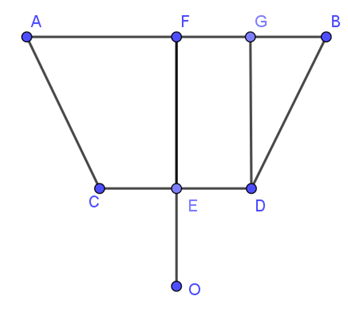
\includegraphics[width=0.32\linewidth]{hinhve/GK1-12-LTT/cau16-loi-giai-hinh-thang.png}
		\end{center}
		$BD=\sqrt{GD^2+GB^2}=\sqrt{\left(\dfrac{\sqrt{2}}{x^2}\right)^2+x^2}$.\\
		Chiều cao mặt bên của khối chóp cụt là
		$$h_1=\sqrt{BD^2-\left(\dfrac{x}{2}\right)^2}=\sqrt{\left(\dfrac{\sqrt{2}}{x^2}\right)^2+x^2-\dfrac{x^2}{4}}=\sqrt{\dfrac{2}{x^4}+\dfrac{3x^2}{4}}.$$
		Bán kính đường tròn ngoại tiếp đáy lớn là:
		$$R^2=(OE+h_1)^2+x^2=\left(x\dfrac{\sqrt{3}}{2}+\sqrt{\dfrac{2}{x^4}+\dfrac{3x^2}{4}}\right)^2+x^2.$$
		Bán kính đường tròn ngoại tiếp đáy lớn đạt giá trị nhỏ nhất khi $x\approx 1{,}07$.
	}
\end{ex}

%%%=============Câu 17=============%%%
\begin{ex}%[GK1, THPT Lý Tự Trọng - Đà Nẵng, 2025-2026]%[VNPmath]%[2D1V3-6]
	Nhà ông An ở gần bờ kênh ông dự định thiết kế một ao nuôi vịt như sau: ông bắc một chiếc cầu thứ nhất từ nhà tại điểm $A$ đến điểm $M$ trên bờ kênh. Tại $M$ ông rào một ao hình tròn có đường kính bằng $MC$ và bắc thêm một cây cầu thứ hai từ $M$ đến một điểm $D$ trên bờ ao. Hằng ngày ông đi từ nhà ra kênh trên cây cầu thứ nhất rồi từ đó đi qua cái cầu thứ $2$ rồi đi theo cung tròn của cái ao đến chuồng vịt tại $C$ để cho vịt ăn. Hỏi độ dài của cây cầu thứ nhất là bao nhiêu km, biết ông đi quãng đường dài nhất với góc $\widehat{AMD}=120^{\circ}$ và nhà ông cách bờ kênh $200$ m, $HC=1$ km (kết quả làm tròn đến hàng phần trăm).
	\begin{center}
		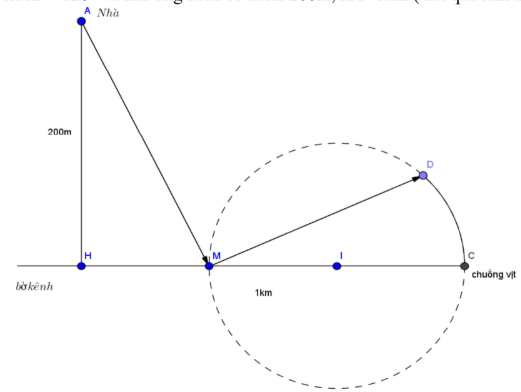
\includegraphics[width=0.6\linewidth]{hinhve/GK1-12-LTT/cau17-hinh-hoc.png}
	\end{center}
	\shortans{0{,}30}
	\loigiai{
		Đáp số: 0,30.\\
		$AH=200$ m $=0{,}2$ km.\\
		Đặt $\widehat{DMC}=x$, $\widehat{AMH}=\dfrac{\pi}{3}-x$.\\
		Suy ra $AM=\dfrac{0{,}2}{\sin\left(\dfrac{\pi}{3}-x\right)}$, $HM=0{,}2\cot\left(\dfrac{\pi}{3}-x\right)$,\\
		$\Rightarrow DM=MC\cos x=\left[1-0{,}2\cot\left(\dfrac{\pi}{3}-x\right)\right]\cos x$.\\
		Độ dài cung $\widehat{DC}=\dfrac{\pi\cdot MC\cdot x}{2\pi}=\left[1-0{,}2\cot\left(\dfrac{\pi}{3}-x\right)\right]\dfrac{x}{2}$.\\
		Quãng đường ông An đi là:
		$$y=\dfrac{0{,}2}{\sin\left(\dfrac{\pi}{3}-x\right)}+\left[1-0{,}2\cot\left(\dfrac{\pi}{3}-x\right)\right]\cos x+\left[1-0{,}2\cot\left(\dfrac{\pi}{3}-x\right)\right]\dfrac{x}{2}.$$
		$y_{\max}\approx 1{,}16098$ khi $x\approx 0{,}305$.\\
		Vậy độ dài của cây cầu thứ nhất là: $AM=\dfrac{0{,}2}{\sin\left(\dfrac{\pi}{3}-x\right)}\approx 0{,}30$ (km).
	}
\end{ex}

%%%=============Câu 18=============%%%
\begin{ex}%[GK1, THPT Lý Tự Trọng - Đà Nẵng, 2025-2026]%[VNPmath]%[2D1V3-6]
	Một nhà máy $A$ chuyên sản xuất một loại sản phẩm cho nhà máy $B$, nhà máy $A$ chỉ bán sản phẩm cho nhà máy $B$ và nhà máy $B$ cam kết thu mua hết số sản phẩm mà nhà máy $A$ sản xuất được. Nhà máy $A$ có khả năng sản xuất được tối đa là $200$ tấn sản phẩm trong $1$ tháng. Nếu bán ra $x$ tấn sản phẩm cho nhà máy $B$ thì giá bán mỗi tấn sản phẩm là $45-0{,}0002x^2$ triệu đồng. Trong một tháng nhà máy $A$ phải chi phí cho nhân công và chi cho khấu hao máy móc một lượng cố định là $150$ triệu đồng, ngoài ra khi sản xuất mỗi tấn sản phẩm thì nhà máy phải chi phí thêm cho mua nguyên liệu là $34$ triệu đồng. Biết rằng nhà máy $A$ phải nộp $6\%$ doanh thu cho cơ quan thuế. Tính lợi nhuận sau thuế (lợi nhuận sau khi đã trừ tiền thuế) lớn nhất thu được trong $1$ tháng của nhà máy $A$ (đơn vị tính là triệu đồng và kết quả làm tròn đến hàng đơn vị).
	\shortans{521}
	\loigiai{
		Đáp số: 521.\\
		Doanh thu một tháng của nhà máy $A$ khi chưa trừ thuế là:
		$$\left(45-0{,}0002x^2\right)x=-0{,}0002x^3+45x\quad(\text{triệu đồng}).$$
		Lợi nhuận sau thuế là: $y=(1-6\%)\left(45x-0{,}0002x^3\right)-150-34x$ (triệu đồng), với $0\leq x\leq 200$.\\
		$y=-0{,}000188x^3+8{,}3x-150$.\\
		$y'=-0{,}000564x^2+8{,}3=0\Rightarrow\hoac{&x\approx 121{,}31\\&x\approx -121{,}31.}$\\
		BBT
		\begin{center}
			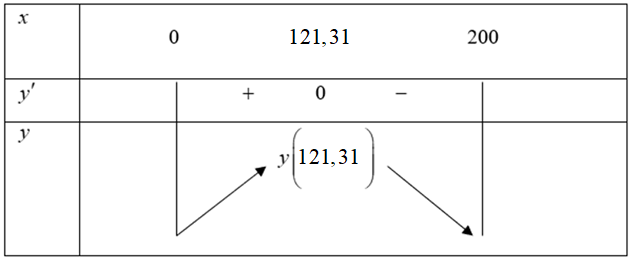
\includegraphics[width=0.62\linewidth]{hinhve/GK1-12-LTT/cau18-bbt.png}
		\end{center}
		Vậy lợi nhuận sau thuế (lợi nhuận sau khi đã trừ tiền thuế) lớn nhất thu được trong $1$ tháng của nhà máy $A$ là $y(121{,}31)\approx 521$ triệu đồng.
	}
\end{ex}

\TL

%%%=============Câu 19=============%%%
\begin{bt}[1,5 điểm]%[GK1, THPT Lý Tự Trọng - Đà Nẵng, 2025-2026]%[VNPmath]%[2D1H5-1]
	Khảo sát sự biến thiên và vẽ đồ thị hàm số $y=-x^3+3x^2-4$.
	\loigiai{
		- Tập xác định $D=\mathbb{R}$.\\
		- Sự biến thiên:\\
		$+$ Ta có $y'=-3x^2+6x$.\\
		Suy ra $y'=0\Leftrightarrow-3x^2+6x=0\Leftrightarrow\hoac{&x=0\\&x=2.}$\\
		$+$ Trên khoảng $(0;2)$, $y'>0$ nên hàm số đồng biến trên khoảng $(0;2)$; trên các khoảng $(-\infty;0)$, $(2;+\infty)$, $y'<0$ nên hàm số nghịch biến trên mỗi khoảng đó.\\
		$+$ Hàm số đạt cực tiểu tại $x=0;y_{\text{CT}}=y(0)=-4$; hàm số đạt cực đại tại $x=2;y_{\text{CĐ}}=y(2)=0$.\\
		$+$ Giới hạn tại vô cực: $\lim\limits_{x\to-\infty} y=+\infty;\lim\limits_{x\to+\infty} y=-\infty$. Hàm số đã cho không có tiệm cận.\\
		$+$ Bảng biến thiên:
		\begin{center}
			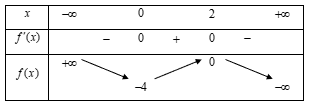
\includegraphics[width=0.55\linewidth]{hinhve/GK1-12-LTT/cau19-bbt.png}
		\end{center}
		- Đồ thị: Giao điểm của đồ thị hàm số với trục tung là điểm $(0;-4)$.\\
		Ta có $y=0\Leftrightarrow-x^3+3x^2-4=0\Leftrightarrow\hoac{&x=-1\\&x=2.}$
		\begin{center}
			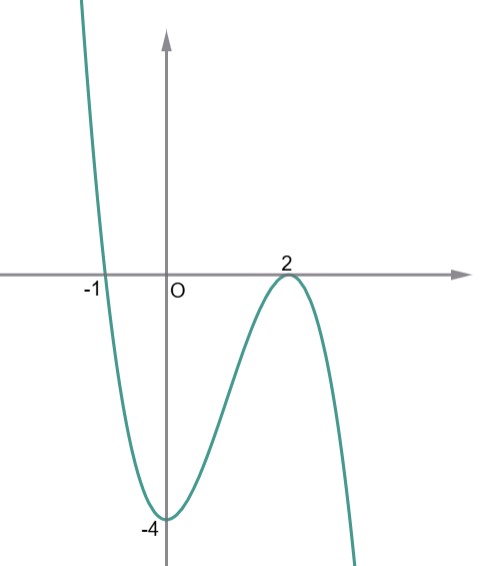
\includegraphics[width=0.42\linewidth]{hinhve/GK1-12-LTT/cau19-do-thi.png}
		\end{center}
	}
\end{bt}

%%%=============Câu 20=============%%%
\begin{bt}[1,0 điểm]%[GK1, THPT Lý Tự Trọng - Đà Nẵng, 2025-2026]%[VNPmath]%[2D1H3-1]
	Tìm giá trị lớn nhất và giá trị nhỏ nhất của hàm số $y=-x^4+4x^2+6$ trên đoạn $[-1;4]$.
	\loigiai{
		Ta có $y'=-4x^3+8x$.\\
		Khi đó $y'=0\Leftrightarrow-4x^3+8x=0\Leftrightarrow\hoac{&x=0\in(-1;4)\\&x=\sqrt{2}\in(-1;4)\\&x=-\sqrt{2}\notin(-1;4).}$\\
		Khi đó: $y(-1)=9$; $y(0)=6$; $y\left(\sqrt{2}\right)=10$; $y(4)=-186$.\\
		Do đó $\max\limits_{x\in[-1;4]} y=y\left(\sqrt{2}\right)=10$; $\min\limits_{x\in[-1;4]} y=y(4)=-186$.
	}
\end{bt}

%%%=============Câu 21=============%%%
\begin{bt}[0,5 điểm]%[GK1, THPT Lý Tự Trọng - Đà Nẵng, 2025-2026]%[VNPmath]%[2D1N3-1]
	Một vật chuyển động theo quy luật $s=-2t^3+24t^2+9t-3$ với $t$ là khoảng thời gian tính từ lúc bắt đầu chuyển động và $s$ là quãng đường vật đi được trong khoảng thời gian đó. Tính vận tốc của vật lúc $t=4$?
	\loigiai{
		Ta có vận tốc tức thời $v(t)=s'(t)=-6t^2+48t+9$.\\
		Khi đó $v(4)=105$.
	}
\end{bt}

\Closesolutionfile{ans}

\inputansbox{12,2,4}{ans/ans\currfilebase}
